% ----------------------------------------------------------------------^
% Copyright (C) 2004, 2005, 2006, 2007, 2008 Giorgio Calderone
% (mailto: <gcalderone@ifc.inaf.it>)
% 
% This file is part of MCS.
% 
% MCS is free software; you can redistribute it and/or modify
% it under the terms of the GNU General Public License as published by
% the Free Software Foundation; either version 2 of the License, or
% (at your option) any later version.
% 
% MCS is distributed in the hope that it will be useful,
% but WITHOUT ANY WARRANTY; without even the implied warranty of
% MERCHANTABILITY or FITNESS FOR A PARTICULAR PURPOSE.  See the
% GNU General Public License for more details.
% 
% You should have received a copy of the GNU General Public License
% along with MCS; if not, write to the Free Software
% Foundation, Inc., 51 Franklin St, Fifth Floor, Boston, MA  02110-1301  USA
% 
% ----------------------------------------------------------------------$


\documentclass[12pt,titlepage]{article}

\usepackage[english]{babel}
\usepackage{graphicx}
\usepackage{framed}
\usepackage{listings}

\usepackage{a4wide}
\usepackage{fancyhdr}
\pagestyle{fancy}
\renewcommand{\footrulewidth}{0.4pt}

%LN
%\renewcommand{\sectionmark}[1]{\markright{\thesection.\ #1}}
%\renewcommand{\sectionmark}[1]{\markright{#1}}
%\renewcommand{\subsectionmark}[1]{\markright{#1}}
%\parindent 0pt


%\textheight 22cm
%\textwidth 16.5cm
%\topmargin 0cm
%\oddsidemargin -0.5cm
%\evensidemargin -0.5cm
%\sloppy

\newcommand{\mcs}{\textbf{MCS} }
\newcommand{\myro}{\textbf{MyRO} }
\newcommand{\dif}{\textbf{DIF} }
\newcommand{\votpp}{\textbf{VOTPP} }

\def\ver{Ver. \input{../version}}
\def\url{http://ross.iasfbo.inaf.it/mcs}

\newcommand{\syntax}[1]
{
  \bigskip
  \noindent
  \textbf{Syntax: } \\
  \indent \texttt{#1}
}

\newenvironment{parameters}
{
  \bigskip
  \noindent
  \textbf{Parameters:}
  \begin{enumerate}
}
{
  \end{enumerate}
}

\newcommand{\param}[2]
{
  \item \textit{#1} \texttt{#2}
}

\newcommand{\return}[1]
{
  \bigskip
  \noindent
  \textbf{Return value} (\texttt{#1}): \\
  \indent
}

\begin{document}

%
%Listing package:
%http://www.pvv.ntnu.no/~berland/latex/docs/listings.pdf
%
\lstloadlanguages{[ISO]C++}
\lstset{
  language=c++,
  frame=leftline,
  escapeinside={//(}{)},
  morekeywords={string},
  basicstyle=\footnotesize,
  keywordstyle=\bfseries, stringstyle=\ttfamily, commentstyle=\textit,
  numbers=left, numberstyle=\tiny, stepnumber=1, numbersep=5pt,
  showstringspaces=false, emphstyle=\underbar,
  captionpos=b,
  aboveskip=3mm,
  belowskip=3mm,
  xleftmargin=0.5cm,
  emph={
        TINY,SMALL,MEDIUM,INT,BIGINT,FLOAT,DOUBLE,STRING,TIME,TINY_BLOB,BLOB
        ,AccumBuffer
        ,B64_Codec
        ,BaseThread
        ,Binary
        ,Client
        ,ClientInfo
        ,Column
        ,CommandParser
        ,Conf
        ,Coosys
        ,Data
        ,DBConn
        ,Definitions
        ,Description
        ,Dynamic_Array
        ,Element
        ,Env
        ,Event
        ,Field
        ,FieldRef
        ,Fits
        ,Group
        ,HostInfo
        ,Info
        ,Link
        ,LocalThread
        ,Max
        ,Min
        ,NetInterface
        ,NodePointer
        ,Option
        ,Param
        ,ParamRef
        ,Parser_Stream
        ,Parser_Table
        ,Parser_Tree
        ,Pipe
        ,Query
        ,Record
        ,RecordSet
        ,Resource
        ,Row
        ,Serializable
        ,Server
        ,ServerSocket
        ,Socket
        ,Stream
        ,Synchro
        ,Table
        ,Tabledata
        ,Thread
        ,URLReader
        ,UserThread
        ,Values
        ,VOTable
        ,VOTableReaderSplit
        ,Writer_Stream
        ,mcs
        ,mcsStart
        ,mcsWait
        ,mcsCustomStart
        }
}


%LN
%\lhead[\sectionmark]{{\bfseries MCS: user manual}}
%\lhead[\rightmark]{\rightmark}
%\rhead{\thepage}
%\chead[]{}
%\lfoot[]{}
%\cfoot[\sl MCS user manual]
%      {\sl MCS user manual}
%\rfoot[]{}
%\setlength{\headrulewidth}{0.4pt}
%\setlength{\footrulewidth}{0.4pt}


\title{
%
\textbf{MCS \\ My Customizable Server}
%
%\thanks{\url}
%
\begin{center}
\vspace{0.1cm}
\includegraphics[width=6cm,keepaspectratio]{mcslogo} \\
\vspace{0.1cm}
\end{center}
%
\centerline{\rule{\textwidth}{0.4pt}}
%
}
\bigskip
\author{
  \sc{Giorgio Calderone} \\
  %\footnote{Giorgio Calderone $<$gcalderone@ifc.inaf.it$>$}  \\
  \sc{IFC - INAF Palermo, Italy} \\ \\
  \sc{Luciano Nicastro} \\
  %\footnote{Luciano Nicastro $<$nicastro@iasfbo.inaf.it$>$} \\
  \sc{IASF - INAF Bologna, Italy} \\
 }
\date{\today \\
      \ver \\
      \url \\
      \centerline{\rule{\textwidth}{0.4pt}}
     }
\maketitle

\thispagestyle{empty}
~

\vfill
{\it\small This page intentionally left blank.}

\newpage
\pagenumbering{roman}

\tableofcontents

\newpage
%\lstlistoflistings

\newpage
\pagenumbering{arabic}
%\mainmatter

%
%
%---------------------------------------------------------------------
\newpage
\section{Introduction}

\mcs is a collection of high level C++ classes and functions designed
to easily implement the following kind of applications:

\begin{itemize}
\item multi-thread applications;
\item network applications (through TCP);
\item database (MySQL) applications;
\item information servers;
\item VOTable\footnote{through the VOTPP package} and/or FITS access.
\end{itemize}

Aside from these tasks \mcs provides several other features that can be
used to solve common problems when developing applications in C++. The
greatest advantage in using \mcs is that it exploits the C++ capabilities
in developing high-level tasks but does not require the developer to deal
with networking, threading, database code, or in general low-level code.
Furthermore some repetitive tasks like converting data between
different types or creating and manipulating dynamically allocated data
structures can be easily accomplished using the \mcs classes.

\bigskip
\mcs has been developed on the GNU/Linux platform and it is released under the
GPL license. It can be freely downloaded from the site \textsf{\url}. This
site contains all news, updates, documentation and downloadable software
packages. The site is still under development, so check for updates.

\bigskip
The \mcs project was developed at IFC-INAF (Palermo, Italy)
by Giorgio Calderone and Luciano Nicastro (now at IASF-INAF, Bologna).


\subsection{Motivations}
Information services can be separated in two classes: those in which
the information produced are addressed to humans, and those in which
they are meant for the use by other software applications. In the
former case there is a quite standardized way to develop such an
information service, essentially based upon a web server, a database
server, a scripting language and HTML pages. In the latter case
instead there is no such standardization, and this is one of the
reasons why \mcs (My Customizable Server) was implemented. Thanks to
its communication protocol indeed \mcs can be used to easily develop
information services that can be accessed from other software
applications. Furthermore \mcs provides several mechanisms to customize
the server behaviour and integrate already existing applications. So
\mcs is an attempt to standardize the developing of these kind of
applications. By comparison \mcs and its protocol are for software
applications what a web server and HTTP are for the WWW: a simple way
to access data.

\bigskip
Another reason that drove the development of \mcs is the need in
today's astronomical projects of computational systems capable to
store and analyze large amounts of scientific data, to effectively
share data with other research Institutes and to easily implement
information services to present data for different purposes
(scientific, maintenance, outreach, etc.). Due to the wide scenario of
astronomical projects there isn't yet a standardized approach to
implement the software needed to support all the requirements of a
project. The new approach we propose here is the use of a unified
model where all data are stored into the same database becoming
available in different forms, to different users with different
privileges.

\bigskip
Finally, \mcs has been developed with the goal to simplify C++
developing through the use of high-level classes that relieve the
developers from repetitive tasks. One of the most remarkable example
of this higher level abstraction layer are the \textbf{Data},
\textbf{Record} and \textbf{RecordSet} classes (see Sect.
\ref{sec:The data abstraction layer}).

\bigskip
\mcs is the evolution of a software named SDAMS (SPOrt Data Archiving
and Management System) %\cite{sdams}
that was implemented to support the SPOrt experiment, %(\cite{sport})
an Italian Space Agency (ASI) funded project which has been ``frozen''
because of the problems with the Columbus module on the International
Space Station. At that time the approach used to build SDAMS seemed to
be easily portable to other experiments so its features and usability
have been generalized until it became the actual \mcs. In fact it is
now used to manage the data collected by the optical and infrared
cameras ROSS/REMIR
%(\cite{ross})
mounted on the robotic telescope REM % (\cite{rem})
at La Silla, Chile. %(see Nicastro \& Calderone, this volume)
Although \mcs has been developed to build an information server to
support an astronomical project, it is completely general purpose and
can be used in the same manner in many other kind of projects.
%
%
%MCS is a set of software tools aimed at easily implement information
%services, that is an application that provides a service over the
%network. At the core of a MCS-based system there is a TCP server which
%listen for user connections, and once a user is connected it will send
%all the requested information. However the transmitted data aren't in
%free format (like in a web page), but are packed in a well defined
%fashion (using the MCS protocol) so that on the other side a software
%can understand what is being sent. The MCS high level classes will
%hide all code implementations related to multi-threading, networking,
%database access, etc., and require no low-level knowledge of these
%issues by the users. MCS can also be customized through the derivation
%of some classes.

%
\subsection{\mcs features}
\label{sec-mcs features}
The \mcs classes can be used to simplify application development in
a variety of situations. Anyway we have to warn the reader about the
fact that the \mcs library is not supposed to be used as a system
library replacement: if your application needs a low level control
upon processes, threads, sockets, database connections, data
conversions and memory allocation you simply have to use the system
libraries. Only in this way indeed you can dispose of all the
possibilities offered by the operative systems and the C++ language.
However this kind of applications are just a minor part of all the
applications, thus if your application needs to deal with this topics
from a higher level then you can use the higher-level \mcs classes
instead of the low-level system routines.

\bigskip
The tasks that can be accomplished by the \mcs classes can be subdivided
in the following categories:

\subsubsection{Multithreading applications}
The \textbf{Thread} class can be used to create threads, that are
separate path of execution running in the same process memory
space. To create a separate thread you simply have to derive the
\textbf{Thread} and implement the \textbf{run} method, which will
became the body of execution of the separate thread. Synchronization
between separate threads can be accomplished using the
\textbf{Synchro} class. This class is also used as parent class for
other classes such as \textbf{Record}, which acts as a shared resource
between different threads.

%
\subsubsection{Network applications}
\mcs provides several classes to develop network applications. The
\textbf{HostInfo} class can be used to retrieve information about a
network host, such as its IP address, while the \textbf{NetInterface}
class can be used to retrieve information about the network
interfaces installed on a computer. The \textbf{Socket} class is
capable to open TCP sockets against remote hosts and send data through
it. The \textbf{ServerSocket} can be used to open a server socket,
that is a socket that waits on a specified port for incoming user
connections. This class has been used to implement the \mcs server,
while \textbf{Socket} class has been used to implement the
\textbf{Client} class which can connect to an \mcs server.

%
\subsubsection{The \mcs data abstraction layer}
The \textbf{Data}, \textbf{Record} and \textbf{RecordSet} classes can
be used as a high-level abstraction layers upon data. Basically these
classes offer a unique interface to access data from different
sources (database, files, information sent by the \mcs server,
etc.). Furthermore they provide facilities to convert data between
different formats, serialize data structures, implement thread-safe
queues etc... These classes are intensively used to pass data between
\mcs classes. See Sect. \ref{sec:The data abstraction layer}.

%
\subsubsection{Database access}
The \textbf{DBConn} and \textbf{Query} classes provide the
possibility to connect to a database server (actually only
MySQL\footnote{http://www.mysql.com} is supported but other database
server may be supported in the future) and execute queries on it. Data
can be read from the database and written on it using the \mcs data
abstraction layer.

%
\subsubsection{FITS file access}
The \textbf{FITSReader} class can be used to read a
FITS\footnote{http://heasarc.gsfc.nasa.gov/docs/heasarc/fits.html} file. Data
will be read through the data abstraction layer.


%
\subsubsection{Application server}
An application server is an application that provides a service over
the network. Typically a user connects to the service and issues a query
that will be executed on the server, then the resulting data will be
sent back to the user using a dedicated communication protocol. This
process is very similar to the request of a web page. The \mcs library
provides an already working multithreaded TCP server like many others,
but the \mcs one has two interesting feature:

\begin{itemize}
\item the server behaviour is customizable (that's the reason for its
  name), that is the kind of queries that can be executed can be tuned
  on developer's needs.

\item the communication protocol is perfectly integrated with the
  \mcs data abstraction layer, so that data sent back from the
  server are in a well defined format (not like those of a web page)
  and thus it is very simple to implement an application that can
  access the service.
\end{itemize}


%
\subsubsection{Other facilities}
\mcs has also a lot of minor features that help the developers to deal
with common problems. Two of these facilities are:
\begin{itemize}
\item \textbf{CommandParser}: a class to parse a command line, with
  option and arguments support;

\item \textbf{Conf}: a class to read and write configuration files,
  like the Windows \verb|INI| files.
\end{itemize}


%
\subsubsection{Facilities included in previous releases}
\label{sec:previous:facilities}
A number of other facilities had been part of \mcs in previous
releases. Now these facilities had become separate projects because
they don't depend upon \mcs (except for \textbf{VOTPP}).

\paragraph{\myro (My Record Oriented privilege system)}
\hspace{1cm} \newline \myro\footnote{http://ross.iasfbo.inaf.it/myro} is the
name we use to refer to a technique used to implement a database privilege
system on a per-record basis. Actually all database servers implement
privilege systems based on tables or columns, that is if a user has grants to
access a certain table (or a table column) he can access all records of that
table (or that table column). \myro lets you specify grants on a record level
so a user can access only those records it is allowed to. A consequence of
this is that different users reading the same table will see different
records. The grants mechanism provided by \myro is similar to that of a Unix
file system, that is each record has an ``owner'' and a ``group'' to which the
record belongs. Furthermore it has three sets of permissions (for the owner,
the group, and all other users) that specify if that record can be read and/or
written. The software components of \myro are a Perl script used to perform
administrative tasks, a C library and a set of MySQL functions. The process of
protecting tables is completely transparent to the final user, that is once
\myro has been installed and configured by the database administrator users
can access the database without even know that \myro is working.

%
\paragraph{Astronomy related facilities}
\hspace{1cm} \newline
The most important Astronomy facility is the possibility to read
VOTable\footnote{http://www.ivoa.net/Documents/latest/VOT.html} through the
\textbf{VOTPP}\footnote{http://ross.iasfbo.inaf.it/votpp} (VOTable C++ Parser)
library. VOTable files can be read using the \textbf{Parser\_Stream} or the
\textbf{Parser\_Tree} class, that is using the SAX model (read one node at a
time) or the DOM model (read the entire file and build a browseable tree in
memory). Note that \textbf{VOTPP} provides a distinct class for each possible
VOTable node, so that the C++ code will be very close to the XML counterpart.

\smallskip

Another important Astronomy feature is
\dif\footnote{http://ross.iasfbo.inaf.it/dif} (Dynamic Indexing
Facility) which integrates the
HTM\footnote{http://www.sdss.jhu.edu/htm/} and
HEALPix\footnote{http://healpix.jpl.nasa.gov} indexing facilities
inside database tables. This means that a query involving spherical
coordinates (both in 2D or 3D environments) can take advantage from
the database built-in indexing mechanisms to speed-up execution of a
query.

%\bigskip
%
%The packages relative to these facilities are still distributed with
%\mcs. You can enable the compilation of these facilities using the
%options to the \verb|configure| script (see Sect.
%\ref{sec:configuremcs}).
%



%
\subsection{Using \mcs from other programming languages}
\mcs also provides an interface to use some of its classes from
programming languages other than C++. The features exported through
this interface are:
%
\begin{itemize}
\item the possibility to use the database related classes together with the
  data abstraction layer;
\item the possibility to connect to an \mcs server.
\end{itemize}
%
Due to the fact that not all languages support the object-oriented programming
paradigm what is exported are just functions. An interesting feature of these
functions is that they all have the same names in all languages.

\smallskip
\noindent
Supported programming languages are:
%
\begin{itemize}
\item C;
\item Fortran 77;
\item PHP;
\item Python;
\item IDL.
\end{itemize}
%
Support for Java and Perl will be added soon.

%\subsection{The \mcs server}
%\mcs is a set of C++ high level, easy to use classes aimed at
%implementing an application server, that is an application that
%provides a service over the network. Its main features are the
%possibility to customize the server behaviour through the derivation
%of some classes, and the usage of a well defined communication
%protocol (the \mcs protocol).
%
%\bigskip
%%
%With \mcs you can easily implement custom services on top of
%which different users can perform requests to a common database
%through several tools obtaining different types of data, depending on
%the tool used and the user permissions. The \mcs protocol and software
%tools let user applications obtain data in a well defined binary
%fashion or plain text, so that they are ready to be further processed.
%
%Information servers based upon \mcs can be implemented
%without worrying about TCP connections, multi-threading, database code
%and so on. You only need to focus on the main problem, and write just
%the code needed to realize the tasks that characterize the service to
%your needs. Some of other features of \mcs are:
%
%\begin{itemize}
%\item easy to configure;
%\item authentication and grant support;
%\item database access;
%\item base commands set, support to create new customized commands;
%\item accessibility from other languages such as C, Fortran, IDL, PHP, etc.;
%\item logging facility, etc.
%\end{itemize}
%
%\bigskip
%%
%Furthermore, many \mcs's classes such as \verb|Thread|, \verb|Socket|,
%\verb|Query|, etc., are general purpose so that you can use them also
%in non-server applications. Though these are high level classes, and
%so very easy to use, they're not intended to be an exhaustive
%framework to work with threads, sockets, and so on (for these tasks
%there are already a number of software packets around, such as
%CommonC++, wvStreams, etc.).
%
%
\subsection{License issues}
\label{sec-license}
\mcs is distributed free of charge and according to the GNU General
Public License. This means that you may copy this software and
distribute it free of charge, as well as modify it provided that you
retain this note and mention the authors name. The GNU General Public
License comes with this package in a file named COPYING, for more
information about this license visit \verb|http://www.gnu.org|.

%
%
\subsection{Some simple examples}
\label{sec-somesimpleexamples}
The directory \verb|share/examples| in the \mcs package contains several
examples that can be compiled and executed once \mcs has been installed. To
compile the examples simply execute \verb|make| in that directory.

\bigskip
\noindent
This section is aimed at giving a first sight at the code you should
deal with if you decide to use \mcs. Some aspects may appear unclear
here but these are just examples. Check the following sections for
further and more complete references.

\medskip
\noindent
In the first example (see List. \ref{code:data1}) we'll show
how to set and retrieve information from a \textbf{Data} object, which
is the object upon which is built the entire data abstraction layer.
Note in particular how the \textbf{Data} object takes care of all
the necessary conversions between different data type.

\lstinputlisting[float=hbtp,
                 caption={Source of data1.cc},
                 label={code:data1}]
{../share/examples/data1.cc}
\normalsize

\medskip
\noindent
In the second example (see List. \ref{code:db1}) we'll execute
a query on a database table, and print the result on standard output.
We'll also show how to retrieve data through the data abstraction
layer which, in this case, is implemented by the \textbf{Query} class
(from line \ref{code:db1_line} to the end).

\lstinputlisting[float=hbtp,
                 caption={Source of db1.cc},
                 label={code:db1}]
{../share/examples/db1.cc}

\medskip
\noindent
In the third example (see List. \ref{code:server1}) we'll
build the simplest \mcs application server, without any customization
but with all base features available (authentication support, base
commands, database access, file download and upload, access to
external programs).

\lstinputlisting[float=hbtp,
                 caption={Source of server1.cc},
                 label={code:server1}]
{../share/examples/server1.cc}

\medskip
\noindent
Finally in our fourth example (see List. \ref{code:client1}) we
use the \textbf{Client} class to connect to a running \mcs server
(like the one in the previous example), issue some commands to upload
and download a file and finally execute a query on the remote database
and print the result on standard output.
%
\lstinputlisting[float=hbtp,
                 caption={Source of client1.cc},
                 label={code:client1}]
{../share/examples/client1.cc}
%
You should notice that lines from \ref{code:client1_line} to the end are
exactly the same as those in listing \ref{code:db1}, lines from
\ref{code:db1_line} to the end. This is due to the fact that both the
\textbf{Client} and \textbf{Query} classes implement the data abstraction
layer, thus these classes provide the same interfaces to retrieve data, even
if in one case data are being read from a database, and in the other data have
been packed, sent through the network and then unpacked.

%
%
\subsection{About this document}
\label{sec:aboutthisdocument}
This document gives an overview of the \mcs facilities and focuses on
some of the basic topics of \mcs. It is divided in several sections so
that you can read only the information you need:
\begin{itemize}

\item \textbf{\mcs installation and usage}: it provides information about
  the configuration of the package against all optional dependencies,
  the compilation and installation, furthermore it shows how to link
  against the \mcs library;

\item \textbf{Developer's manual}: it introduces the reader to some of the
  \mcs basic concepts like the data abstraction layer, thread
  handling, database connections, etc., and focuses on various
  techniques to develop applications with \mcs;

\item \textbf{The \mcs server}: it shows how to implement, customize,
  execute and administrate an \mcs server;

\item \textbf{Client's manual}: it shows how to connect to an \mcs
  server;

\item \textbf{Using \mcs with other programming languages}: describes
  all the available interfaces to connect to \mcs through other
  languages;

\item \textbf{libmcs reference}\footnote{available only in HTML format
    at: \textsf{\url}}: technical description of the \mcs library
  implementation. It is produced using
  \textsf{Doxygen}\footnote{http://www.stack.nl/$\sim$dimitri/doxygen/}.
\end{itemize}

\smallskip
\noindent
The \mcs documentation is \emph{work in progress}, so you should
always look for the last version. If you find any errors we'd
appreciate if you could send us an email\footnote{Giorgio Calderone
  $<$gcalderone@ifc.inaf.it$>$, Luciano Nicastro
  $<$nicastro@iasfbo.inaf.it$>$}. A users' mailing list is being
prepared, so please contact us if you are a potential user. Thanks in
advance.

%
%---------------------------------------------------------------------
\newpage
\section{\mcs installation and usage}
The \mcs software library is distributed in a \verb|tar.gz| package.
You can find the latest version at \textsf{\url}. To unpack the package simply
issue the command:
%
\begin{verbatim}
    tar xvzf mcs-x.y.z.tar.gz
\end{verbatim}
%
where \verb|x|, \verb|y|, \verb|z| are the version number (namely the
first number is the major revision, the second number is the version,
and third number is the subversion). A directory named
\verb|mcs-x.y.z| will be created containing all sources code as well
as the documentation and the scripts needed to install \mcs. Before
installing \mcs you should check that all mandatory dependencies are
satisfied (see Sect. \ref{sec:Dependencies}), then you must follow a
three step procedure: Configure, Compile and Install.

\subsection{Dependencies}
\label{sec:Dependencies}
The only mandatory packages required by \mcs are:

\begin{itemize}
\item Perl (http://www.perl.com, version 5.8.5 or later);
\item PCRE (http://www.pcre.org, version 6.4 or later);
\item cURL (http://curl.haxx.se, version 7.12 or later).
\end{itemize}

\noindent
Typically these packages are already installed in the system, if this
is not the case you should install them before continuing. However
there are a lot of \mcs facilities which depend on other optional
packages:

\begin{itemize}
\item MySQL (http://www.mysql.com/, version 5.1 or later): used to
  connect and manage a database, to handle client authentications and grants;

\item Openssl (http://www.openssl.org/, version 0.9.7 or later): used
  to implement secure connections through sockets;

\item CFITSIO (http://www.cfitsio.org/, version 0.9.7 or later): used
  to read data in FITS format;

\item IDL (http://www.ittvis.com/idl/, version 5.6 or later): used to
  implement the IDL to MCS interface;

\item PHP (http://www.php.net/, version 5.0.5 or later): used to
  implement the PHP to MCS interface;

\item Python (http://www.python.org/, version 2.3 or later): used to
  implement the Python to MCS interface.

\noindent
You can enable or disable the compilation of each facility with the
corresponding option of the configure script (see Sect.
\ref{sec:configuremcs}).
\end{itemize}

%
\subsection{Installing \mcs}
\label{sec:installing}

%
\subsubsection{Configure}
\label{sec:configuremcs}
Configuring \mcs means checking your system for compatibilities,
search for include files and libraries, and finally produce all
necessary \textsf{Makefile}s needed to compile \mcs. This is done
automatically by the distributed \verb|configure| script. Typically
you can use this script without any option, as follows:

\begin{verbatim}
    ./configure
\end{verbatim}

\noindent
Anyway \verb|configure| has a lot of options and switches (type
\verb|configure --help| for a list) to customize the compilation step.
The options like \verb|with-PACKAGE=PATH| can be used to specify the
path where the \verb|configure| script should search to find that
package (default is \verb|/usr/local|). Some of these options are
specific to \mcs:

\begin{itemize}
\item \verb|--prefix=PATH| \\
  the directory under which all include files, libraries and other
  files relative to \mcs will be installed, if this option is not used
  \verb|usr/local| is assumed;

\item \verb|--enable-debug, --disable-debug| \\
  if enabled then the "-g" and "-O0" flags will be added to the
  compiler command line; these are needed to include debugging
  information in the library and to discard any optimization. By
  default this option is disabled;

\item \verb|--enable-all| \\
  by default all optional facilities are disabled, you can enable them
  with the relative options (discussed below), or you can enable all
  of them with this option. Note also that if you want to enable all
  option except, say, the interface to Python, you can simply use the
  following arguments: \verb|configure --enable-all --disable-python|.

\item \verb|--with-pcre=PATH| \\
  if the PCRE package (which is mandatory) is not installed in a
  standard location (typically \verb|/usr/local|) then you can provide
  the correct path with this option;

\item \verb|--with-curl=PATH| \\
  if the cURL package (which is mandatory) is not installed in a
  standard location (typically \verb|/usr/local|) then you can provide
  the correct path with this option;

\item \verb|--enable-mysql, --disable-mysql, --with-mysql=PATH| \\
  enable or disable the compilation of MySQL facilities, by default
  this option is enabled;

\item \verb|--enable-openssl, --disable-openssl, --with-openssl=PATH| \\
  enable or disable the compilation of Openssl facilities, by default
  this option is disabled;

\item \verb|--enable-cfitsio, --disable-cfitsio, --with-cfitsio=PATH| \\
  enable or disable the compilation of CFITSIO facilities, by default
  this option is disabled;

\item \verb|--enable-idl, --disable-idl, --with-idl=PATH| \\
  enable or disable the compilation of IDL to \mcs interface, by default
  this option is disabled;

\item \verb|--enable-php, --disable-php, --with-php=PATH| \\
  enable or disable the compilation of PHP to \mcs interface, by default
  this option is disabled;

\item \verb|--enable-python, --disable-python, --with-python=PATH| \\
  enable or disable the compilation of Python to \mcs interface, by default
  this option is disabled;
\end{itemize}

\bigskip

%\noindent
%The \mcs distribution also contains other packages whose compilation
%can be enabled using the following options:
%%
%\begin{itemize}
%\item \verb|--enable-myro| \\
%  enable or disable the compilation of \myro (My Record Oriented
%  privielge system) package, by default this option is disabled;
%
%\item \verb|--enable-dif| \\
%  enable or disable the compilation of \dif (Dynamic Index Facility)
%  package, by default this option is disabled;
%\end{itemize}
%%
%Documentation for these packages is available on their own web sites
%(see Sect. \ref{sec:previous:facilities}).

\noindent
There are several other options and switches available, for further
documentation see the \verb|INSTALL| file.

%
\subsubsection{Compile}
\label{sec:compilemcs}
To compile \mcs, once the \verb|configure| script has been correctly
executed, simply issue the command:
%
\begin{verbatim}
    make
\end{verbatim}
%
If you got errors while compiling check Sect. \ref{sec:configuremcs}
and the \verb|INSTALL| file.

%
\subsubsection{Install}
\label{sec:installmcs}
If \mcs has been correctly compiled you can install with the command:
%
\begin{verbatim}
    make install
\end{verbatim}
%
If your account doesn't have the permission to write in the
path where it should be installed then you'll get an error. In this case you
should login as ``root'' and retry.



\subsection{Troubleshooting}
In this section we show solution to the most common problems
encountered while configuring and compiling \mcs.

%\subsection{Problems while configuring}
%%
%\subsection{Problems with CFITSIO}
%\subsection{Problems with libxml}
%\subsection{Problems with MySQL}
%\subsection{Problems with OpenSSL}
%\subsection{Problems with PCRE}
%%
%\subsection{Problems with Fortran}
%\subsection{Problems with IDL}
%\subsection{Problems with PHP}
%
\subsubsection{Problems with Python}
To build the Python to \mcs interface the Python include files are
required. These are available in the Python source distribution or in
the ``Python devel'' package of your distribution.

\begin{itemize}
\item The header \verb|Python.h| has not been found: a symbolic link
  named \verb|python| must point to the actual Python includes
  directory, and it must be located either in \verb|/usr/include| or
  \verb|/usr/local/include|.
%Questo perche' nel codice generato da SWIG si cerca il file
%"python/Python.h"
\end{itemize}




%
\subsection{Using the \mcs library}
Once you have installed the \mcs library (see Sect. \ref{sec:installing}) you
can use it in your C++ code as described here.

\subsubsection{Include \mcs header}
All \mcs classes and functions are defined inside the \verb|mcs| namespace to
avoid conflict with other libraries you may use. To use the \mcs facilities
you must include the \mcs header in your C++ source code as follows:
%
\begin{verbatim}
    #include <mcs.hh>
    using namspace mcs;
\end{verbatim}
%
To use the \mcs library with other programming languages see Sect. \ref{Using
  mcs with other programming languages}.

%
\subsubsection{Compile and link}
The \mcs package installs a script named \verb|mcs-config| which can be
used to retrieve several information regarding the installation
itself, for example the location of the include files and of the
libraries, as well as the list of the libraries to link to:
%
\begin{verbatim}
    mcs-config --cflags
    mcs-config --libs
\end{verbatim}
%
For all other options type \verb|mcs-config --help|. To compile and
link a program (whose source file is, say, \verb|myprog.cc|) against
the \mcs library you can issue the commands:
%
\begin{verbatim}
    cpp `mcs-config --cflags` -c myprog.cc
    cpp -o myprog myprog.o `mcs-config --libs`
\end{verbatim}
%
or with a single command:
%
\begin{verbatim}
    cpp `mcs-config --cflags` myprog.cc -o myprog `mcs-config --libs`
\end{verbatim}
%
Note that the single quotes are ``reversed single quotes'' (ASCII
decimal code 96).


%
%---------------------------------------------------------------------
\newpage
\section{Developer's manual}
This section is aimed at showing to the reader some of the \mcs
basic concepts like the data abstraction layer, thread
handling, database connections, etc., and focuses on various
techniques to develop applications with \mcs. We will often refer to
classes, methods and function whose complete documentation can be
found in the \mcs library reference \footnote{\textsf{\url}}.

%
\subsection{The data abstraction layer}
\label{sec:The data abstraction layer}
The data abstraction layer is a set of classes aimed at providing a
uniform access to data coming from different sources, and to easily
manipulate and transmit those data. Namely the classes involved are
\textbf{Data}, \textbf{Record} and \textbf{RecordSet}, with each one
representing a different level of data hierarchy.

\subsubsection{The \texttt{Data} class}
\label{sec:The Data class}
The first level corresponds to the \textbf{Data} class, which can be
used to store a single data, that is a number, a string, a date/time,
a binary object, etc. The main feature of a \textbf{Data} object is
its capability of performing conversions between different types of
data, that is you can assign to a \textbf{Data} object different types
of data, as in the following example:

\begin{lstlisting}
//Create a Data object
Data mydata(STRING, 20);

//Assign an integer.
mydata = 12;

//Assign a floating point number.
mydata = 1.2;

//Assign a string
s = "My name is Giorgio";
\end{lstlisting}

\noindent
As you can assign different type of data to a \textbf{Data} object,
you can also assign a \textbf{Data} object value to different types
of variable, as in the following example:

\begin{lstlisting}
//Assign to an integer variable
int i = mydata.ival();

//Assign to a floating point variable
float f = mydata.fval();

//Assign to a string variable
string s = mydata.sval();
\end{lstlisting}

\noindent
You should have noticed that in this case a simple assignment is not allowed,
so you have to call the appropriate \verb|*val()| method of the \textbf{Data}
class, in which the first character is \verb|i| for integers, \verb|f| for
single precision floating point numbers, \verb|s| for strings, etc. Note
however that a \textbf{Data} object is not a ``dynamic type'' object (like
those of other programming languages such as Perl, PHP, IDL), indeed it always
has a ``base type'' that determines the size of its internal buffer and the
behaviour of the different conversion routines (in the last example the ``base
type'' is a string 20 characters long). A consequence of this fact is that an
assignment can also lead to an error, just because the ``base type'' cannot
change during the use of the object and some conversions do not make sense. In
our previous example, assigning a string more than 20 characters long would
have led to an error. Let's examine another case where an assignment could
lead to an error:

\begin{lstlisting}
//Create a Data object with base type INT
Data mydata(INT);

mydata = 12;  //Ok
mydata = 1.2; //Ok, will be rounded to 1
mydata = 1.5; //Ok, will be rounded to 2

mydata = "A string"; //Error!!! //(\label{intro_Data_error1})
mydata = "123";      //That is correct. //(\label{intro_Data_ok1})

int i = mydata.ival();     //Ok, i = 123
string s = mydata.sval();  //Ok, s = "123"
\end{lstlisting}

\noindent
As you can see the assignment in line \ref{intro_Data_error1} doesn't
make any sense, you can't assign a generic string to an integer base
type. On the other hand the assignment in line \ref{intro_Data_ok1} is
perfectly allowed because that string can be converted to an integer.
Finally, the last two assignment are allowed, even if in the first
case the variable will be set to a value of \verb|123| as an integer,
whereas in the second the variable will be set to the string
\verb|"123"|, whose memory representation is quite different from the
integer in the first case.

\subsubsection{The \texttt{Record} class}
\label{sec:The Record class}
On the second level of hierarchy there is the \textbf{Record} class
which can be seen as a dynamically-sized array of \textbf{Data}
objects. Here the word ``record'' is meant in the sense of a record in
the Pascal language or the struct in C/C++; indeed a \textbf{Record}
object can contain any number of \textbf{Data} objects of any base
type. Creating and populating a \textbf{Record} is quite simple:

\begin{lstlisting}
//Create a Record object
Record rec;

//Create some Data objects
Data d1(STRING, 20);
Data d2(INT);
Data d3(TIME);

//Give a name to the Data objects
d1.setName("A_String");
d2.setName("An_Integer");
d3.setName("A_Float");

//Add the Data objects to the Record objects
rec.addField(d1);
rec.addField(d2);
rec.addField(d3);

//Now we can refer to each Data object using the syntax
//we would use with any C/C++ array
rec[0] = "Hello";
rec[1] = 123;
rec[2] = 1.23;
Data& tmp = rec[0];

//We can also refer to a Data object using its name.
string s = rec["A_String"].sval(); //(\label{code:example_record_line})
int    i = rec["An_Integer"].ival();
float  f = rec["A_Float"].fval();
\end{lstlisting}

\noindent
As can be seen from the example a \textbf{Record} object can be used
like a usual C/C++ array, that is using square brackets(\verb|[]|).
Another interesting feature which links the \textbf{Data} and
\textbf{Record} classes is the possibility to give a name to the
\textbf{Data} object and use that name to search the object inside a
\textbf{Record} object (see line \ref{code:example_record_line} in
previous example).

\subsubsection{The \texttt{RecordSet} class}
\label{sec:The RecordSet class}
The third level of hierarchy is the \textbf{RecordSet} class, which is a
dynamically-sized container of \textbf{Record} objects. It is not required
that all contained objects have the same structure (that is the same sequence
of base type for \textbf{Data} objects). Using a \textbf{RecordSet} object is
quite similar to using a file handler, indeed there is a current
\textbf{Record} object pointed by a cursor (like a pointer to a record in a
file) that can be moved forward and backward in the file to search for the
required data. The following example shows how to populate a
\textbf{RecordSet} object, and how to visit all the contained \textbf{Record}
objects:

\begin{lstlisting}
//Create a RecordSet object
RecordSet rset();

//Insert the Record object created in the previous example
rset.insert(rec);

//Insert other Record objects as needed...
rset.insert(...);

//Visit all Record objects

//To visit all Record objects we have to move to the first
//Record object in the set
rset.setFirst();

//Loop through all Record objects in the set
while (! rset.eof()) {
  //Get a reference to the current Record object
  Record& r = rset.rec();

  //Use the record in some way...

  //Move to the next Record object in the set.
  rset.setNext();
}
\end{lstlisting}

\noindent
The previous example, however, shows a quite rare usage of the
\textbf{RecordSet} class, in fact it would be useless to populate a
record and read it again inside the same programming unit. The most
common way to populate a \textbf{RecordSet} is to derive the class and
overload the \verb|fetch()| virtual method. As an example see the code
of the \textbf{FileReader} class.

\bigskip
It is worth to mention that, while the names ``record'' and
``recordset'' are often used in database terminology, the
\textbf{Record} and \textbf{RecordSet} classes are not limited to
database access, instead they are designed to be general purpose. For
example the \textbf{RecordSet} is the parent class of the
\textbf{Parser\_Table} class, which is used to read VOTable files. Of
course these classes are also used to perform database access, in
particular the result of a query inside the \mcs library is presented
as a \textbf{RecordSet} object, a record of the result is presented as
a \textbf{Record} object and a field of the record is presented as a
\textbf{Data} object. Another important feature of these classes is
that they implement the \textbf{Serializable} interface, so they can
be easily sent through the network using the \textbf{Socket} class.
Indeed all message passing between client and server during an \mcs
session is performed using these objects to incapsulate the
information being sent.

%
\subsection{Threads and synchronization}
\label{sec:Threads and synchronization}
Threads are essentially identical copies of a code which run on
different data, and let your program perform several ``contemporary''
tasks. \mcs lets you implement code that runs in separate threads, and
it provides a way to synchronize those threads using the \textbf{Thread}
and \textbf{Synchro} classes.

\subsubsection{The \texttt{Thread} class}
\label{sec:The Thread class}
To implement a code which runs in a separate thread you should derive
the \textbf{Thread} class and overload its virtual \verb|run()|
method. This will become the body of execution of the separate thread.
Suppose you want to implement an application which reads file names
from standard input and ``contemporary'' perform some task on the
given files. The derived class would be as in the following example:

\begin{lstlisting}
//A ``global'' queue, while file names are read from stdin they
//are stored in this queue.
Record queue;

//Derive the Thread class
class MyThread : public Thread {

  void run() {
    for (;;) {
      //If there's at least one file name in the queue...
      if (queue.count()) {
        string fn = queue.pop().sval();
        //...perform some task on the file
      }
      sleep_ms(1000); //wait for one second.
    }
  }
};
\end{lstlisting}

\noindent
As you can see this thread waits until there are file names in a queue,
and once the data arrive it will take the file name and perform some
task on the file. The main program should read the file names from
stdin, as in the following example:

\begin{lstlisting}
int main() {
  //Create the thread object and start it...
  MyThread t;
  t.start();

  string s;
  while (cin >> s) //Read from standand input
    queue.push(s); //Insert the string in the queue
}
\end{lstlisting}

\noindent
This program will always be ``alive'' that is it will always react
when you type a filename on stdin, even if it is working on a file in
a separate thread.

\bigskip
The \textbf{Thread} class is used inside \mcs to implement the multithreaded
server. In the simplest case, when a user connects to the server it will
create an instance of a class named \textbf{UserThread} (which derives
\textbf{Thread}) which will listen for user commands and eventually will send
back the requested data.  Thus the main server program can continue to listen
for new users connections. Also, if other users are already connected, they
will have their own thread to work with.  This way the server can provide
services to different users at the same time.

\subsubsection{The \texttt{Synchro} class}
\label{sec:The Synchro class}
Once you have different threads running in your application you may
need to synchronize them. A typical example occurs when the threads
need to access a global variable. Suppose that in the previous
example the computation inside the thread is very time consuming, and
you want to elaborate two files in parallel. This can be easily done
creating two (or even more) instances of the \verb|MyThread| class in
the main program:

\begin{lstlisting}
  //Create two instances of the MyThread class.
  MyThread t1;
  MyThread t2;

  //Start separate threads.
  t1.start();
  t2.start();
\end{lstlisting}

\noindent
That's all is needed to implement the parallel elaboration of two
files. But there's is a hidden bug in this code, what would happen if
both threads try to read from the global queue at the same time?
Even if this is unlikely to occur, both threads could read the same
data from the queue and start the elaboration of the same file, thus
probably leading to an error. This bug can be removed using the
\textbf{Synchro} class to implement ``protected sections'', that are
sections of code that can be executed by only one thread at a time. The
changes in the code are as follows:

\begin{lstlisting}
class MyThread : public Thread {
  //Use the same Synchro object in all parallel threads.
  static Synchro syn;

  void run() {
    for (;;) {
      if (queue.count()) {
        syn.enter(); //Enter the protected section
        string fn = queue.pop().sval();
        syn.leave(); //Leave the protected section
        //...perform some task on the file
      }
      sleep_ms(1000); //wait for one second.
    }
  }
};
\end{lstlisting}

\noindent
As you can see the global variable now is being used inside a
protected section, thus the previous bug cannot occur anymore. Note
also that the protected section is leaved before working on the file,
that is because otherwise the other thread couldn't advance until
the first has ended its job.

%\subsection{Serialization}
%\label{sec:Serialization}
%TO BE WRITTEN.
%
%\subsubsection{The \texttt{Serializable} class}
%\label{sec:The Serializable class}
%TO BE WRITTEN.


\subsection{Database access}
THe \mcs library can be used to execute SQL queries on a MySQL database. The
classes involved are \texttt{DBConn}, \texttt{Query} and \texttt{Table}.

\subsubsection{The \texttt{DBConn} class}
This class is used to open a database connection and perform authentication,
as in the following example:
%
\begin{lstlisting}
DBConn db;
db.connect("mcstest", "mcstest", "test");
\end{lstlisting}
%
If the connection or authentication fails an exception will be thrown.


\subsubsection{The \texttt{Query} class}
Once a connection to the database has been estblished it is possible to
execute SQL queries on it through the \texttt{Query} class:
%
\begin{lstlisting}
Query qry(&db);
qry.prepare("SELECT * FROM mcstest");
qry.execute();
\end{lstlisting}
%
In this case the query produce a result set which can be retrieved through the
data abstraction layer (because \texttt{Query} derives from \texttt{RecordSet}):
%
\begin{lstlisting}
//Loop through the resulting record set
while (! qry.eof()) {
  //Get a reference to current record
  Record& rec = qry.rec();

  //For each field print its value
  for (int i=0; i<rec.count(); i++)
    cout << rec[i].sval() << "\t";
  cout << endl;

  //Move to next record
  qry.setNext();
}
\end{lstlisting}
%

%
%
%\subsection{\mcs server's related classes}
%TO BE WRITTEN.
%
%\subsubsection{The \texttt{UserThread} class}
%TO BE WRITTEN.
%
%\subsubsection{The \texttt{LocalThread} class}
%TO BE WRITTEN.
%
%\subsubsection{The \texttt{Server} class}
%TO BE WRITTEN.

%
%---------------------------------------------------------------------
\newpage
\section{The \mcs server}

\subsection{Architecture of an \mcs based system}
\label{sec:architecture}
An \mcs based system has four main components (see
Fig. \ref{fig:maincomponents}):

%
\begin{figure}[hbtp]
\begin{center}
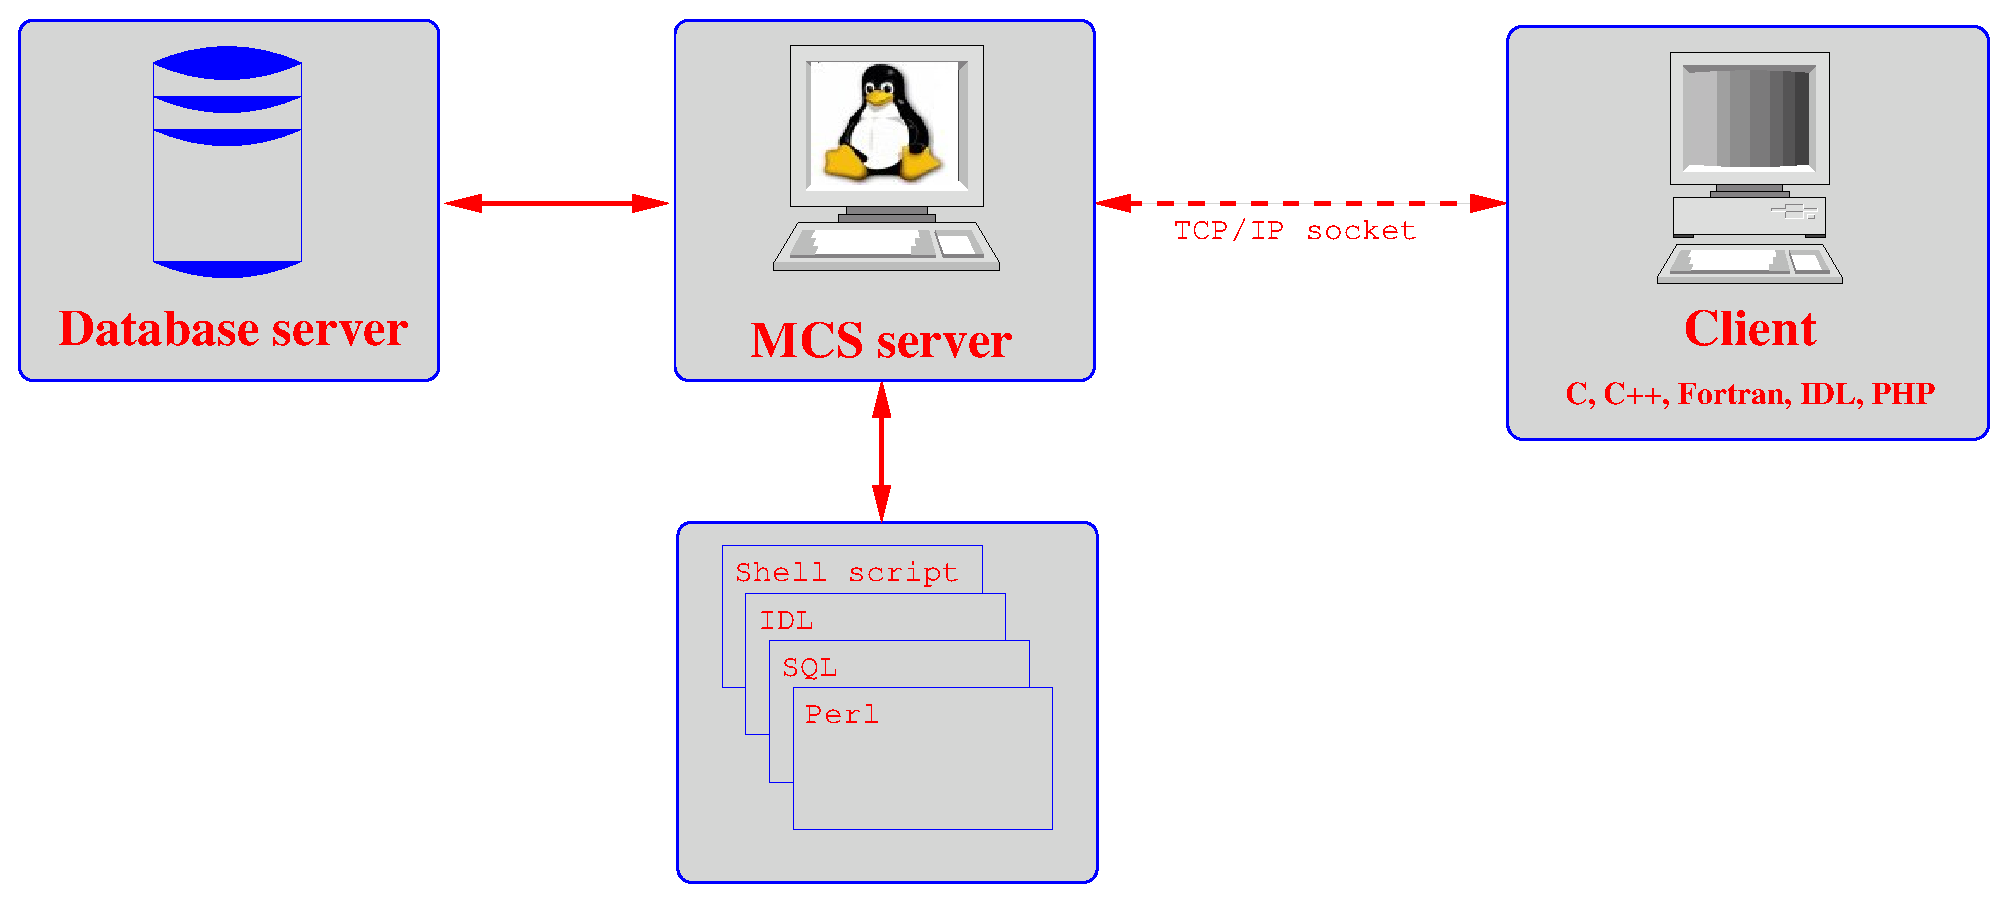
\includegraphics[width=14cm,keepaspectratio]{includes/diaggen}
\end{center}
\caption{Main components of an \mcs based system}
\label{fig:maincomponents}
\end{figure}
%

\subsubsection{Database server}
The database server is used to handle clients authentication, to store
all application specific data and anything else necessary to the
application itself. This server isn't accessible directly from the
clients, but it is visible only to the application server. At the moment
the only supported database server is MySQL \footnote{http://www.mysql.com}.
In the future other servers may become accessible through \mcs.

\subsubsection{Application server (\mcs based)}
The application server is the core of the information system. It
implements the client/server model: a client opens a TCP socket towards
the host running \mcs and sends a request, then the
server ``computes'' an answer, eventually querying the database and/or
executing some external programs, and sends it back to the client.
The behaviour of the \mcs server can be customized deriving some classes.

\subsubsection{External programs}
External programs are software applications written in any language, which
interact with the application server via command line and the standard output.
Support to these programs was added to easily integrate already
existing applications within \mcs.

%
\subsubsection{Clients}
Clients are programs which access the \mcs service over the
network. Such programs can be written in any language and run on any
platform, provided that they implement the \mcs protocol. Interfaces
that implement the \mcs protocol are provided by the \mcs library for
the following languages on the Linux platform: C++, C, Fortran, IDL,
PHP, Python. Support for other languages (such as Java and Perl) and
the Windows platform will be available soon (we hope).

%
\subsection{The \mcs server}
\label{sec:themcsserver}
The \mcs server is an application server, that is an application that waits on
a TCP port until a client gets connected. When a client is connected the
server provides an information service, that is the possibility to request
\emph{information} to the server. Data are transmitted using the \mcs
protocol, which must be implemented by the clients. This protocol is flexible
enough to transmit binary data and files, but also to let a client access the
service offered by \mcs from a simple telnet client . Due to the flexibility
of the protocol, \mcs is the natural solution to implement communication
between different software tools running on different hosts, through the
network. So \mcs can also perform IPC (Inter Process Communication).

%
\subsubsection{Comparison with a ``shell''}
Using interactively an \mcs server resemble very closely the usage of
a classic Unix shell, that is a command line interface with a prompt
on which users can execute commands in their
own environment and wait for the output before a new command can be
issued. It is therefore possible to make a comparison between the
``components'' of a shell, and the ones from an \mcs connection (see
Tab. \ref{paragoneshell}). The concepts listed herein will be
described in details later.

%
\begin{table}[hbtp] \begin{center}
    \bigskip
    \begin{tabular}{|l|l|}
      \hline \textbf{Unix shell} & \textbf{\mcs server} \\ \hline
      \verb|stdin| e \verb|stdout| & bidirectional TCP socket \\
      system account & MySQL account \\ internal commands & base
      commands \\ programs, shell scripts & external programs
      (\verb|EXEC| command) \\ home directory & work directory \\
      \hline
    \end{tabular}
    \caption{``shell'' comparison}\label{paragoneshell}
\end{center} \end{table}
%

\subsubsection{Temporal sequence of events during a connection}
In this section we'll explain the temporal sequence of events during an
\mcs session, using Fig. \ref{flow}.
%
\begin{figure}[hbtp]
\begin{center}
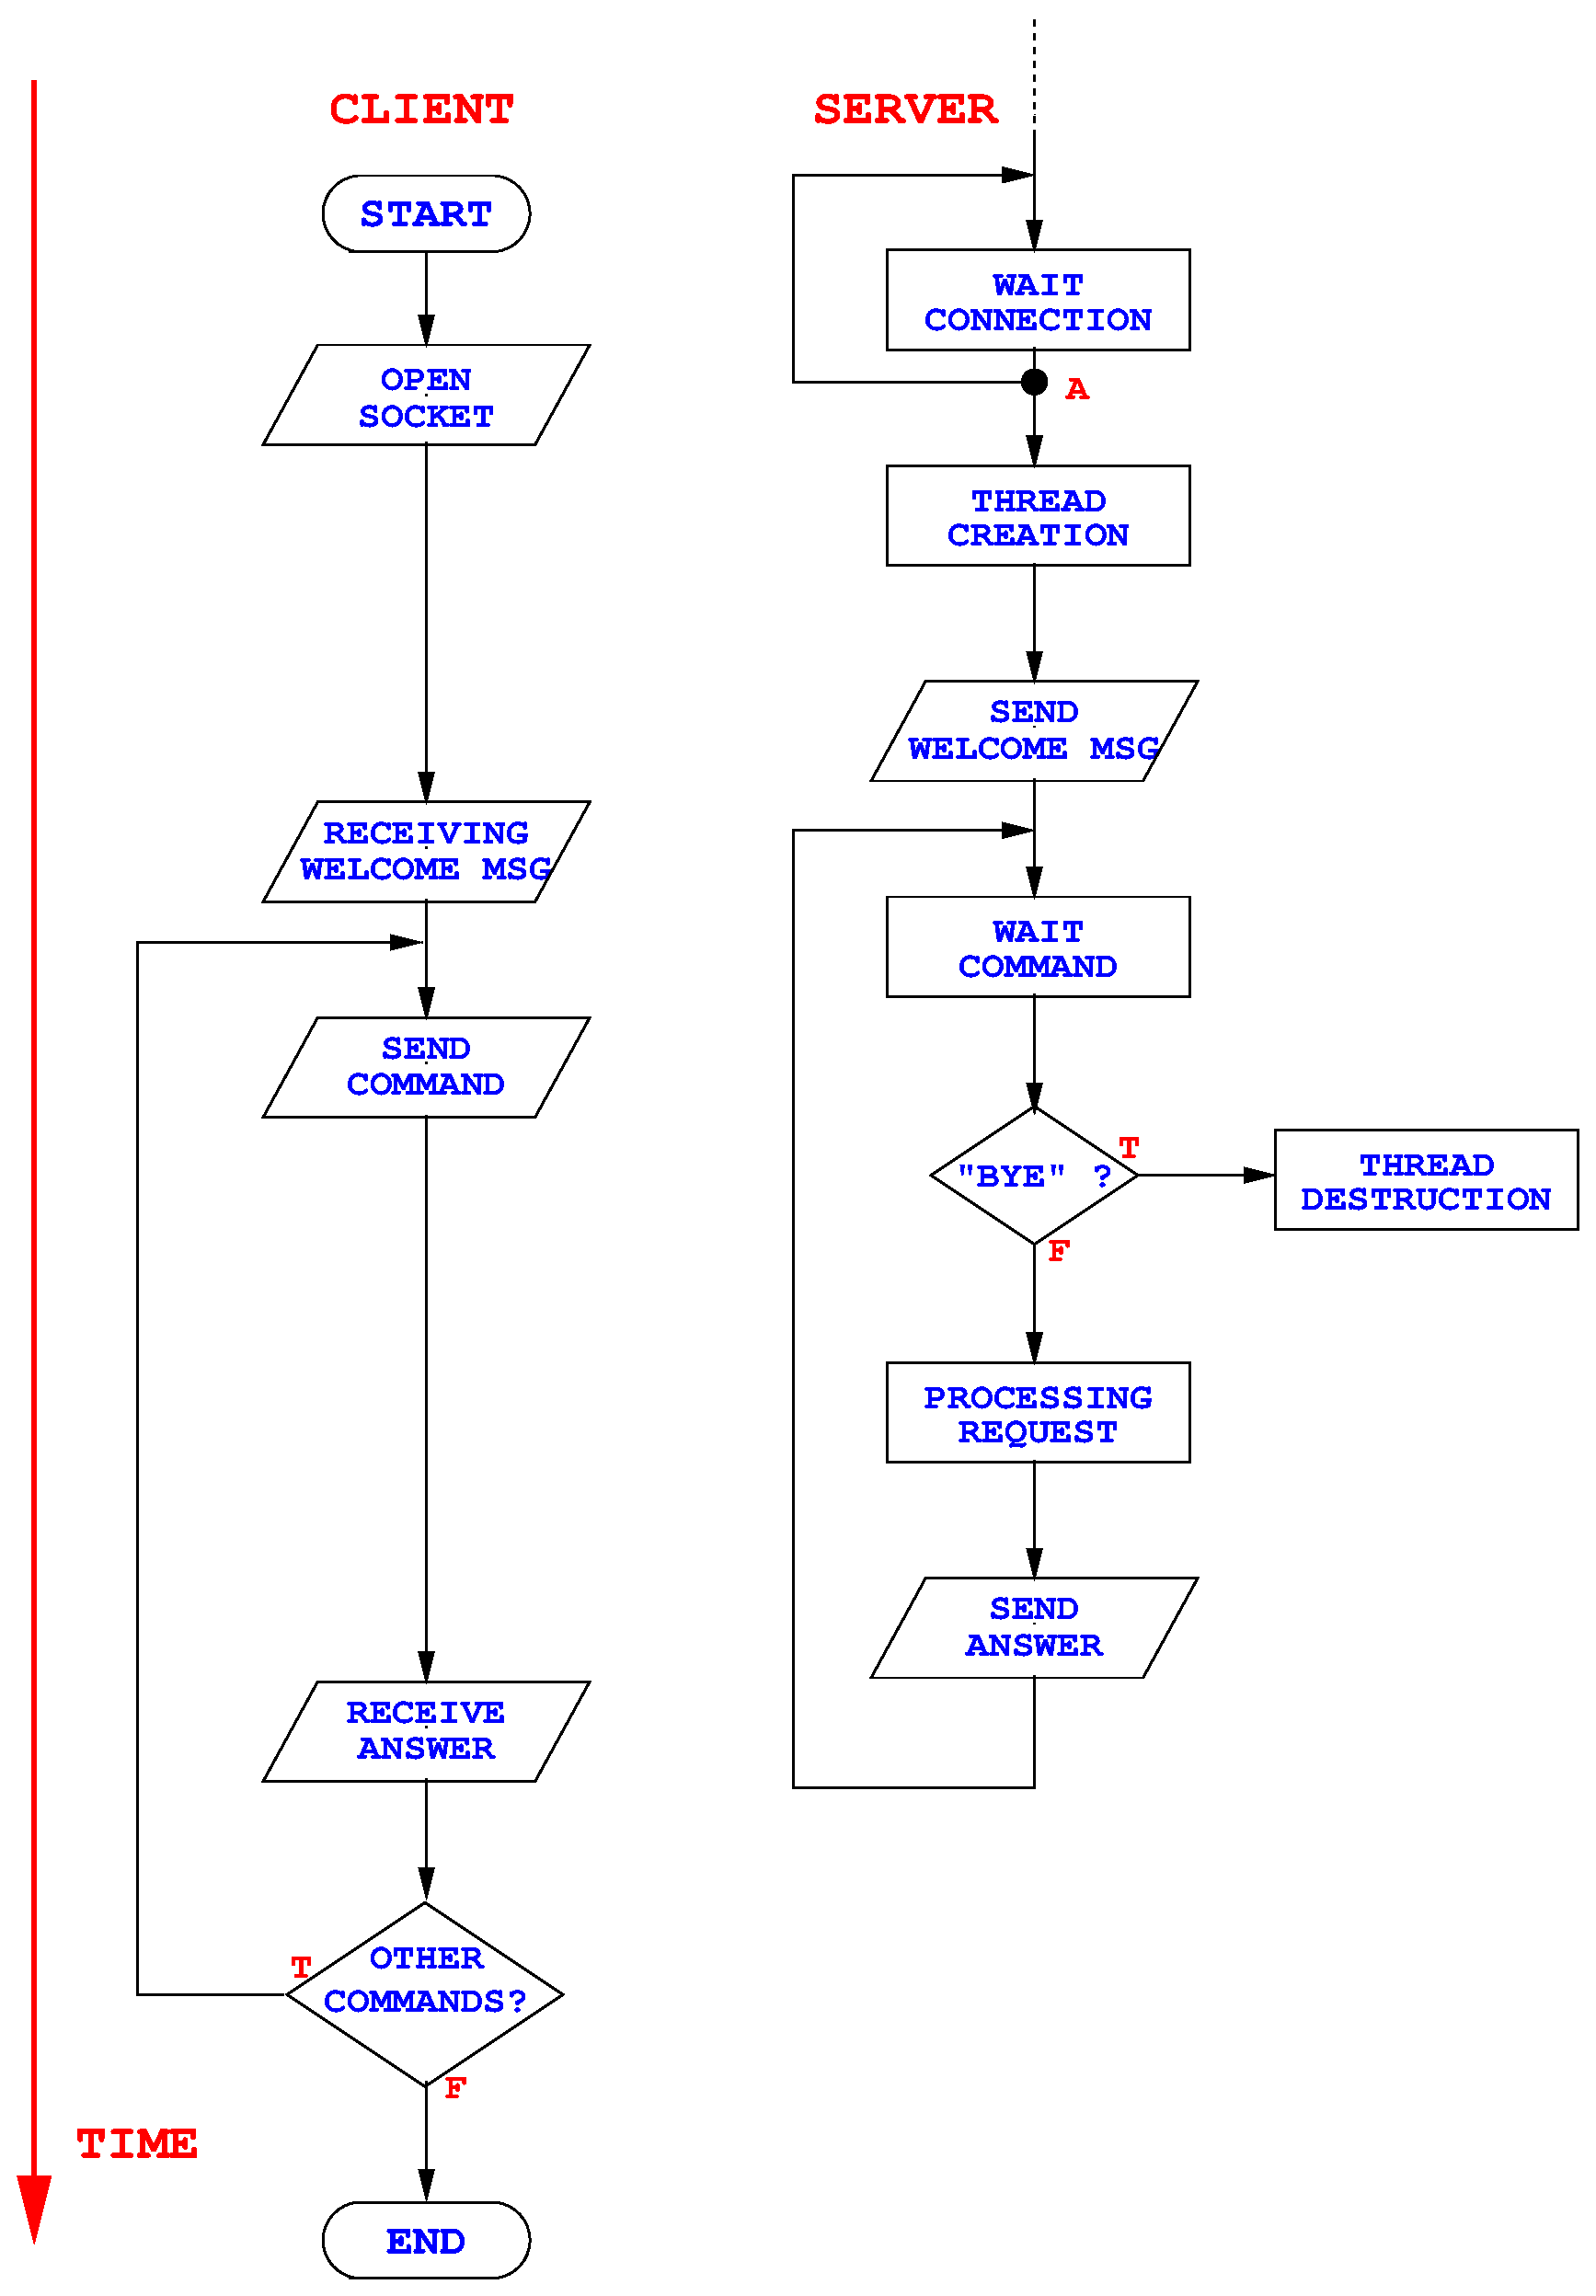
\includegraphics[width=10cm,keepaspectratio]{includes/flow}
\end{center}
\caption{Flow diagram of a typical \mcs session}
\label{flow}
\end{figure}
%
The arrow indicates the time flow; as we can see different
blocks on client and server aren't contemporaries. Furthermore we see
that while for the client the start and end points are well defined,
for the server we don't have such points because we suppose it is
executed indefinitely. Usually the server waits for a client to open a
TCP socket, when such a socket is opened, the server creates a new
thread of execution and assigns the connection to it. We can notice
(point labeled ``A'' in Fig. \ref{flow}), that at this point the
execution path of the server is split in two, one of them returns
to wait for another client, while the other starts processing client
requests on another thread. Threads are basically identical programs
working on different data. In this case the different data are the
different sockets connected to different clients. That's how the server
can process requests from several clients ``simultaneously''.
%
As soon as the new thread is ready, it will send a welcome message
through the socket. Receiving this message indicates that the server
is ready to process client requests. From now on the server will wait
for commands to arrive, while the client will enter a loop to send all
necessary commands and receiving the related answers. When the server
receives a command it will check if it is a \verb|BYE| command, that is
a command to close the connection. If this is the case then the thread
will destroy itself. In all other cases the server will process the request
and send the answer to the client until a \verb|BYE| command is received.

%
\subsubsection{Base commands}
\label{sec:commands}
Users can request a service from an \mcs based application server using
\textbf{commands}. There are two types of commands: \emph{a.}
\textbf{base commands} are those implemented in \mcs itself,
\emph{b.} \textbf{custom commands} are those implemented by the users
(see Sect. ``Developer's manual'').

A command is a sequence of characters terminated by a newline
character, very similar to the ones used in a typical UNIX shell. They
are composed of a keyword (the command itself), zero or more options
(with a ``-'' minus sign) and zero or more arguments, depending on the
command. The command keyword and the options are case insensitive
whereas arguments are not. Options and arguments are separated by one or
more blanks, and can be enclosed in double quotes to be considered as
a single argument (\verb|''a single argument''|). The actual
argument anyway won't contain the double quotes. If an argument must
contain a double quote it can be escaped with a backslash
(\verb|\"|). The Tab. \ref{tabComandi} shows a list of available
\textbf{base commands}. Any base command provides the \verb|-help|
option, which will produce a brief explanation of the command usage.
%
\begin{table}[!hbt]
\begin{center}
\caption{\mcs Command codes}\label{tabComandi}
\bigskip
\begin{tabular}{|l|l|}
  \multicolumn{1}{c}{\textbf{Command code}} &
  \multicolumn{1}{c}{\textbf{Meaning}} \\
  \hline %
  \hline %
\verb|CID    |&Retrieve the CID (Client Identifier)                   \\
\verb|CLINFO |&Retrieve information about all connected clients       \\
\verb|NOP    |&A ``do-nothing'' command                               \\
  \hline %				
  \hline %				
\verb|USR    |&Supply user name                                       \\
\verb|PWD    |&Supply password                                        \\
\verb|DBN    |&Supply application name                                \\
\verb|CON    |&Login                                                  \\
\verb|BYE    |&Close the connection                                   \\
  \hline %
  \hline %
\verb|GET    |&Download a file from work directory                    \\
\verb|PUT    |&Upload a file to the work directory                    \\
\verb|GETDATA|&Retrieve a \verb|Data| object                          \\
\verb|PUTDATA|&Send a \verb|Data| object                              \\
\verb|QRY    |&Execute an SQL query                                    \\
\verb|QRES   |&Send the query result as a file                        \\
\verb|FETCH  |&Retrieve the record at the specified position          \\
\verb|EXEC   |&Execute an external command or script, with parameter  \\
  \hline %
  \hline %
\end{tabular}
\end{center}
\end{table}
%
\noindent A command can be executed each time the \mcs server sends a
prompt, there can be three kinds of prompt:
\begin{itemize}
\item \verb|#0--|: last command executed successfully;
\item \verb|#0W-|: last command report a warning;
\item \verb|#0E-|: last command report an error.
\end{itemize}

%
\paragraph{Options common to all commands}
There are a number of options that are common to all commands, so we
report them here:
\begin{itemize}
\item \verb|-help|: show a brief explanation about the command usage
  and doesn't execute the command;
\item \verb|-force|: continue execution of commands even if an error
  occurred;
\item \verb|-werr|: Turns all warning into errors, so that a warning
  can stop the execution.
\end{itemize}

%
\paragraph{Command \texttt{USR <username>}}
Used to supply the user name to the \mcs server during
authentication. The user name identifies a list of grants. Example:

\bigskip
\verb|usr giorgio|
\bigskip

\paragraph{Command \texttt{PWD <password>}}
Used to supply the password for a specific account. Example:

\bigskip
\verb|pwd my_password|
\bigskip

%
\paragraph{Command \texttt{DBN <application\_name>}}
Used to select the application to which the user wants to connect. This
command can be used when a single \mcs server implements different
applications, otherwise it is not useful. Example:

\bigskip
\verb|dbn test|
\bigskip

This way you will access the application named \verb|test|.

%
\paragraph{Command \texttt{CON}}
This command doesn't need any parameter and it is used to finalize the
authentication process. It must be used after the \verb|USR|,
\verb|PWD| and optionally the \verb|DBN| commands. If the user
authenticates successfully, the following command will be automatically
executed:

\bigskip
\verb|exec auto|
\bigskip

The \mcs server administrator may use the \verb|auto| script to
initialize the user environment.

%
\paragraph{Command \texttt{BYE}}
Logout and close the connection.

%
\paragraph{Command \texttt{CID}}
Every client has a \textbf{Client identifier}, that is a unique
integer number that identifies the associated thread. This command can
be used to retrieve such a number.

%
\paragraph{Command \texttt{QRY [-sqascii] [-sqfits] <query>}}
Execute SQL queries directly on the database DB server. The query
doesn't need to be quoted, and you can use the quotes inside the query
itself. If it is a selection it will return information about the
record set, if it is not will return the number of affected
records. If the option \verb|-sqascii| or \verb|-sqfits| are given
then the result of the query will be written into a file in the work
directory respectively in ASCII or FITS format. Example:

\bigskip
\verb|qry SELECT * FROM table|
\bigskip

\begin{framed}
\bfseries{Notice}: you don't need to supply the '\verb|;|' at the
end of the query, like you would do with the MySQL client.
\end{framed}

%
\paragraph{Command \texttt{QRES}}
This command prepare an ASCII file containing all records from the
last query, then it will send the file to the client.

%
\paragraph{Command \texttt{EXEC <name> [PARS]}}
This command executed an external program, an SQL script or a batch
file. The name of external programs and/or script are specified on the
server in the configuration file. If you're executing an external
program, the parameters will be passed on the command line and its
standard output and error will be written into the work directory in the
\verb|out| and \verb|err| file respectively. If you're executing an SQL
or batch script, the parameters will be substituted inside the script
where a placeholder (like \verb|$1|, \verb|$2|, etc..) is found.
%
%
%\paragraph{Commands \texttt{SQL}, \texttt{SCR}, \texttt{BAT}}
%With these commands it is possible to execute a list of commands (respectively
%in SQL, Shell script, \mcs commands), stored in a file on the application
%server's tree.
%
%Tramite questi codici command \`e possibile eseguire alcune sequenze
%di istruzioni (rispettivamente SQL, Shell script, \mcs)
%memorizzate su un file. Tali script sono parametrizzati in maniera da
%rendere generica la funzionalit\`a offerta. L'esecuzione di questi
%codici command prevede una risposta composta da almeno due
%\textbf{risposte}, indicanti rispettivamente l'inizio e la fine della
%elaborazione. Tra le due \textbf{risposte} di inizio e fine potrebbero
%essere inviate altre \textbf{risposte} (ovvero le risposte ai singoli
%comandi).  Se tra l'inizio e la fine dell'esecuzione avviene un errore
%esso verr\'a segnalato nel modo che compete al command che lo ha
%generato, e l'esecuzione verr\`a bloccata. Anche in caso di errore
%verr\'a comunque trasmessa la \textbf{risposta} finale. Nota che i
%nomi degli script non possono contenere il carattere \verb|'/'| per
%motivi di sicurezza.
%\paragraph{Command \texttt{SCR <script> [PARS]}}
%This command executes a shell script present in the \verb|APPD/usr/scr| or
%\verb|APPD/adm/scr| path (depending if you used the \verb|ADM| switch). An
%example of the syntax is:
%
%\bigskip
%\verb|scr dqry 'T001.T001' '' '10' '1000'|
%\bigskip
%
%This command executes the system command:
%
%\bigskip
%\verb|APPD/usr/src/dquery 'T001.T001' '' '10' '1000'|
%\bigskip
%
%and writes the standard output on \verb|WORK/out|, and standard
%error on \verb|WORK/err|. The \mcs server also replies with the exit code of
%the script, so that the user can see if there was anyz error. The files
%\verb|WORK/out| and \verb|WORK/err| can be retrieved with the \verb|GET|
%command, otherwise thay can be used for another command with the \verb|WRK|
%switch.
%
%\paragraph{Command \texttt{SQL <script> [PARS]}}
%This command executes a sequence of SQL instructions, stored in a file in the
%\verb|APPD/usr/sql| or \verb|APPD/adm/sql| path (depending if you used the
%\verb|ADM| switch). An example of the syntax is:
%
%\bigskip
%\verb|sql getrawtable T001|
%\bigskip
%
%With this command you execute the SQL script \verb|getrawtable|, passing as
%first parameter the string \verb|T001|. If the last query of the script is a
%select-like query then the result can be retrieved with the \verb|QRES|
%command.
%
%%
%\paragraph{Command \texttt{BAT <script> [PARS]}}
%This command execute a sequence of \mcs commands, just like those we are
%dealing with, stored in a file in the
%\verb|APPD/usr/scr| or \verb|APPD/adm/scr| (depending if you used the
%\verb|ADM| switch). An example of the syntax is:
%
%\bigskip
%\verb|bat auto|
%\bigskip
%
%Like with the \verb|SQL| command, we can also use parameters for the batch
%file.

%
\paragraph{Command \texttt{GET [<file\_name>]}}
Retrieve a file located into the work directory on the server. The
parameter is the file name. If no parameter is passed then the file
\verb|out| will be retrieved.

\paragraph{Command \texttt{PUT <file\_name> <size>}}
Store a file into the work directory on the server. Parameters are the
file name and the file size in byte.

%
\subsubsection{Grants}
TO BE WRITTEN.


%
\subsection{Running the \mcs server}
TO BE WRITTEN.

\subsubsection{The configuration file}
TO BE WRITTEN.


%
\subsection{Customize the \mcs server}
\label{sec:customizemcs}
One of the main feature of \mcs (as its acronym suggests) is the possibility
to be customized, adapting the server behaviour to specific needs/tasks.
\mcs can be customized in several ways:

\begin{itemize}
\item adding external programs, either real external applications or
  batch lists of \mcs commands;
\item adding SQL programs, to be executed on the database server;
\item adding customized commands, deriving the \verb|UserThread|
  class;
\item modifying the behaviour of the local thread, deriving the
  \verb|LocalThread| class;
\end{itemize}

We'll explain in detail how to customize the \mcs server in the following
sections.

\subsubsection{Adding external programs}
TO BE WRITTEN.

\subsubsection{Adding SQL scripts}
TO BE WRITTEN.

\subsubsection{Adding BATCH scripts}
TO BE WRITTEN.

\subsubsection{Adding custom commands}
TO BE WRITTEN.

%
%
\newpage
\section{Connecting to an \mcs service}
To connect to an \mcs service you can use one of the available
interfaces for the various languages: C++, C, Fortran, IDL, PHP or Python
(Perl and Java will be added). They already implement all the
features of the \mcs protocol like handling connection and data
transfer, either as a file or as record sets. One of the main features
of these interfaces, as shown below, is that the syntax (except for
the C++ interface) is almost identical for all languages.

\subsection{The Client class}\label{sec:Clientclass}
The \verb|Client| class is the main interface to \mcs; all other
interfaces are implemented through it. We recommend to read the
reference documentation for the classes we'll mention.

\bigskip
%\noindent The Fig. \ref{source:client} shows a simple examples
%of a client program written in C++.
%
%\lagrind[hbtp]{includes/client.cc.tex}{Source of client.cc}
%{source:client}
%
\noindent The \verb|Client| class constructor (line 9) accepts
parameters about \emph{a.} the \verb|CLIPATH| directory (see
Fig. \ref{fig:dirs}),  \emph{b.} the host address of the host whose running the
\mcs service, \emph{c.} the port on which the server is listening. Once you
are connected to the server, you can use the \verb|login()| method (line 11)
to perform authentication and the \verb|exec()| method (line 12) to
issue commands. In this examples we issued the \verb|CID| command to
retrieve the client identifier. Each data exchanged between client and
server passes through one of the public \verb|Record| members of the
\verb|Class| client. In this case the client identifier is contained
into a \verb|Data| object in the \verb|aux| member (line 14). As an
example of another \verb|Record| member we can require a brief help
message about a command (line 16, 17, 18). Then we can perform a query
on the database and print all records (line 20 to 33). Finally we
close the connection and delete the \verb|Client| object (line 35 and
36). Note that all the code is in a \verb|try..catch| block to
eventually catch exceptions that may be thrown (\mcs code throws only
exception based on the class \verb|Event|).



\subsection{User environment}
Once a user has connected and logged in (see Sect. \ref{sec:login}) to
an \mcs service, he/she has a dedicated environment consisting of:
\begin{itemize}
\item a work directory, where the user can upload or download files;
\item a database connection, so that a user can perform database
queries as well as create temporary tables visible only to the user
itself.
\end{itemize}

In this document we will refer to the work directory on the server
with \verb|CLIPATH|. With the same name we'll refer to the directory
on the client side from/to which files are uploaded or downloaded (see
Fig. \ref{fig:dirs}). Figure \ref{fig:dirs} shows a directory called
\verb|SRVPATH| above \verb|CLIPATH|: this is the server main directory
which contains all work directories.
%
%
\begin{figure}[hbtp]
\begin{center}
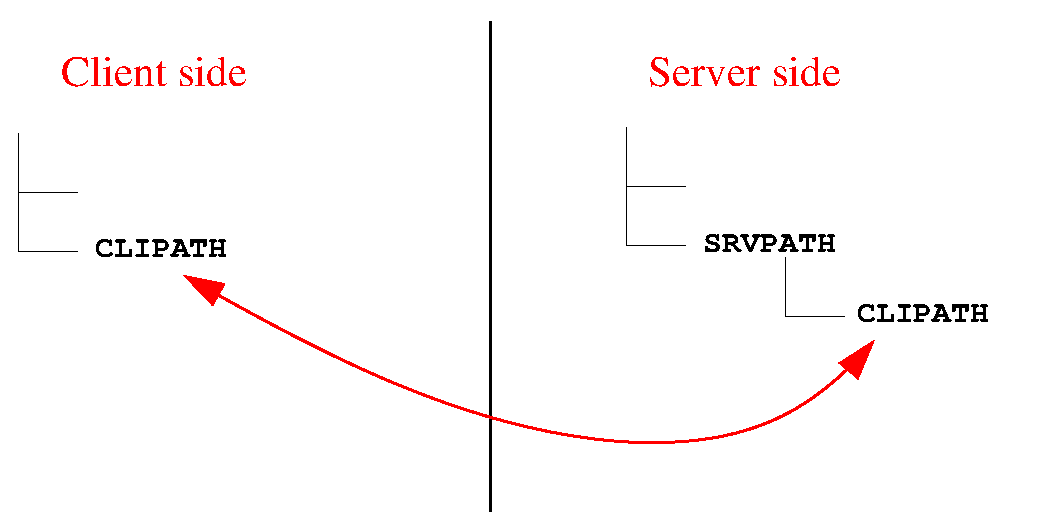
\includegraphics[width=14cm,keepaspectratio]{includes/dirs}
\end{center}
\caption{Directories in an \mcs based system}
\label{fig:dirs}
\end{figure}

%
%
\subsection{Login}\label{sec:login}
The authentication should be made just after the connection using the
\verb|USR|, \verb|PWD|, \verb|DBN| (optional) and \verb|CON| commands.
Some commands (\verb|QRY|, \verb|FETCH|, \verb|EXEC|, etc...) require
the user to be logged in, otherwise a permission error will occur.

\subsection{Logout}\label{sec:logout}
To logout simply issue the command \verb|BYE| then close the
socket. It is important that the client closes the socket first,
otherwise the resource on the server will remain locked.

\noindent When a user closes its connection the server will close the
database connection, destroy the thread associated with the client and
optionally delete all files in the user work directory. (\mcs will
use the \myro package to handle grants).
%
%When a user accesses the service, he/she has a list of grants that allow or deny
%certain operations. If the \verb|read_grants| is set to zero then all users
%have all grants, otherwise grants can be specified on a table named
%\verb|grants|. Possible grants are:
%\begin{table}[!htb] \begin{center}
%    \caption{User's grants}\label{tab:grants1}
%    \bigskip\bigskip
%    \begin{tabular}{|l|l|}
%      \hline
%      \textbf{Symbol} & \textbf{Meaning} \\
%      \hline
%      \verb|MG_NO_GRANTS  | &    no grants       \\
%      \verb|MG_LOGIN      | &    login allowed   \\
%      \verb|MG_SQL_SCRIPTS| &    command SQL	 \\
%      \verb|MG_SCRIPTS    | &    command SCR	 \\
%      \verb|MG_QUERY      | &    command QRY	 \\
%      \verb|MG_BATCH      | &    command BAT	 \\
%      \verb|MG_GET        | &    command GET	 \\
%      \verb|MG_PUT        | &    command PUT	 \\
%      \verb|MG_SYS        | &    command SYS	 \\
%      \verb|MG_ADMIN      | &    command ADM	 \\
%      \verb|MG_ALL        | &    all grants above\\
%      \hline
%    \end{tabular}
%\end{center} \end{table}
%

%---------------------------------------------------------------------
\newpage
\section{Using \mcs with other programming languages}
\label{Using mcs with other programming languages}
An \mcs session is quite similar to a telnet client, so user can
connect to the server also with a simple telnet program. But to take
advantage of all the feature of the \mcs protocol you'll need to use
one of the available interfaces.

\noindent \mcs is written in C++, so most of its facilities are
available as classes. In the following sections we'll assume that the
reader has a minimum knowledge of the object oriented paradigm, as
well as the C++ syntax. Furthermore we'll mention some of the \mcs
classes, whose reference documentation can be found at
%\verb|http://spora.ifc.inaf.it/mcs| or
%\verb|http://ross.iasfbo.inaf.it/mcs|.
\textsf{\url}.

\noindent A user which connects to an \mcs server needs to deal with the
following classes:
\begin{itemize}
\item \verb|Client|: the interface to connect to an \mcs server;
\item \verb|Data|: the base class by which data are exchanged between
  client and server;
\item \verb|Record|: a collection of \verb|Data| objects;
\item \verb|RecordSet|: a collection of \verb|Record| objects.
\end{itemize}
%
Furthermore the following set of classes may be useful to a client
program:
\begin{itemize}
\item \verb|DBConn|: connect to a database server;
\item \verb|Query|: execute queries and retrieve results;
\item \verb|Table|: perform direct access on a database table;
\item \verb|Conf|: reads configuration files.
\end{itemize}

\noindent In Sect. \ref{sec:Clientclass} we'll explain how to write a
program which connects to an \mcs server using these classes and the
C++ language. If a user wishes to use another language to connect to
\mcs he can use one of the available interfaces, which are simply wrappers
to the classes mentioned above. For this reason the code to connect to
\mcs is quite similar in all languages, and we recommend to read
Sect. \ref{sec:Clientclass} also if you don't plan to use
C++. Successive sections will report information specific to each
language. As already mentioned, the languages actually supported are:
C, Fortran, IDL, PHP and Python.
In the near future interfaces will be developed for Java and Perl.
%
%Furthermore we developed a system of C macros, named \textbf{IFD}
%(Interface Descriptor), capable of generating code for a C wrapper to a C++
%library, and to translate a C++ interface to a meta-language. We used
%\textbf{IFD} with the following classes of the \mcs library:
%\begin{itemize}
%\item \verb|MyData|
%\item \verb|MyVector|
%\item \verb|DBFac|
%\item \verb|mcscli|
%\end{itemize}
%So we have a C wrapper to these classes (its interface is in the file
%\verb|mcs_c.h|, and the object code is compiled into the \mcs library).
%
%Other languages can also use \mcs classes through some
%interface. Actually we developed an interface to the following languages:
%\begin{itemize}
%\item \textbf{PHP}: the interface relies upon the C wrapper, and it is
%  automatically generated by a program named \textbf{SWIG}
%  \footnote{www.swig.org};
%\item \textbf{IDL}: the interface relies upon the C wrapper, and it is
%  generated using the meta-language produced by \textbf{IFD} and a Perl
%  program named \verb|c2idl|.
%\end{itemize}
%
%The subject of this Section are the description of all these interfaces
%and their usage.
%

%
%
%
%\section{The Interface Descriptor (IFD)}
%(TO BE WRITTEN)
%
%The \textbf{IFD} is basically a set of C macros contained in the file
%\verb|ifd.h|, installed with \mcs. Its main purposes are to generate a
%C wrapper to some C++ classes, and a meta-language which describes these
%classes. To use \textbf{IFD} you must create an header file which contain the
%description of your C++ code. This description is made using the \textbf{IFD}
%macros as shown in the following files installed with \mcs:
%\begin{itemize}
%\item \verb|MyData_c.h|: description of the interface to class \verb|MyData|;
%\item \verb|MyVector_c.h|: description of the interface to class
%  \verb|MyVector|;
%\item \verb|DBFac_c.h|: description of the interface to class \verb|DBFac|;
%\item \verb|mcscli_c.h|: description of the interface to class \verb|mcscli|;
%\item \verb|mcs_c.h|: includes header needed by the C wrapper, and all the
%  above files.
%\end{itemize}
%
%The interface should contain all constructors and destructor of the
%classes you wish to use.
%
%Macros which describes the interface are the following:
%\begin{itemize}
%\item \verb|IFD_CONSTRUCTOR(CLASS, CPARS)|: to describe a class constructor,
%  its parameters are the name of the class
%							
%IFD_COPY_CONSTRUCTOR(CLASS)
%							
%IFD_DESTRUCTOR(CLASS)
%
%IFD_WRAP(RETTYPE, CLASS, METHOD, CALL)
%
%IFD_WRAP_VOID(CLASS, METHOD, CALL)
%
%IFD_C_WRAP(RETTYPE, FUNCTION, CALL)
%
%IFD_C_WRAP_VOID(FUNCTION, CALL)
%\end{itemize}

%
\subsection{Interface usage and naming convention}
In this section we describe how to use the interfaces for languages
others than C++, and the naming convention used. For a detailed
description of all the classes involved and their methods check the
reference manual as well as Sect. \ref{sec:Clientclass}.

\bigskip
As mentioned above, the interfaces are simply wrappers around C++
classes, so when you're calling a function of the interface in your
favourite language, you are actually calling a method of a C++ object
that lives in the heap (dynamic) memory. That's the reason why there
isn't a reference documentation for each interface, the main reference
for the \mcs classes contains all the information you need. Note
that not all the class members are wrapped in the various interfaces
(because only C++ supports overloading), check the classes
documentation to see if a method is wrapped or not. To use the
interface you should therefore create an object, call one or more of
its methods and finally destroy him.

\bigskip
Before using an object you must call the appropriate wrapper to the
constructor which returns the memory address where the object has been
allocated. You should not modify this address, neither modify the type
of the variable where the address has been stored (for those languages
that let you do this), otherwise the object will become
unreachable. We recommend to destroy objects when they are no longer
needed. You can do this by calling the appropriate wrapper to the
destructor and passing the address of the object to be destroyed. The
memory address you got from the constructor must also be passed to all
the wrappers to methods of that class.

\begin{framed}
\textbf{Important note:} What is returned by the wrapper to
constructor routine is just a memory address, so the language you are
using (even C!)  doesn't know anything about the type of object that
has been created. For this reason, if you use this address with a
wrapper of another class, your compiler won't give you any compilation
or syntax error but you will likely get a ``segmentation fault'' when the
program is running.
\end{framed}

\noindent There is only one exception to this rule: if an object
derives from other classes then you can use the address of that
object also with wrappers of parent classes.

\noindent In the following sections we'll explain the naming
convention for a generic class named \verb|CLASS|. Arguments in
brackets (\verb|<>|) are specific to a function or method. Arguments
named \verb|addr| are the memory address of an object.

\subsection{Constructors}
\label{ssec-Constructors}
Constructors follow the name convention:
%
\begin{verbatim}
  addr = new_CLASS(0, <PARAMETERS>)
\end{verbatim}
%
where the parameters are the ones needed by the constructor. The first
parameter is reserved for future use. Note that only one constructor
can be wrapped so check the documentation to see which one is
used. These functions return the memory address where the object has
been allocated. You must use this address in the subsequent methods
call. In all interfaces this memory address is stored in a numeric
variable, you should avoid changing its value or the type of the
variable.

%
\subsection{Copying constructors}
Copying constructors follows the name convention:
%
\begin{verbatim}
  newaddr = copy_CLASS(addr)
\end{verbatim}
%
These functions don't need any specific parameter but only the address
of the object to be copied. Note that you should call the appropriate
copy constructor (the one belonging to the same class with which the
object was created), otherwise you will surely get a ``segmentation
fault''. These functions return the memory address of the newly created
object.

\begin{framed}
\textbf{Note:} actually only the \verb|Data| class has a copy
constructor implemented in the interfaces at the moment.
\end{framed}

%
\subsection{Destructors}
\label{ssec-Destructors}
Destructors follows the name convention:
%
\begin{verbatim}
  del_CLASS(addr)
\end{verbatim}
%
These functions don't need any specific parameter but only the address
of the object to be destroyed. Note that you should call the
appropriate destructor (the one belonging to the same class with which
the object was created), otherwise you will surely get a ``segmentation
fault''. These functions doesn't return any value.

%
\subsection{Methods}
\label{ssec-Methods}
Methods follow the name convention:
%
\begin{verbatim}
  retval = CLASS_methodname(addr, <PARAMETERS>)
\end{verbatim}
%
where the parameters are the ones needed by the method. Note that
because overloading is not supported, only one method with a certain
name can exist. The type and meaning of the returned values depend on
the method called; check the class documentation.

\subsection{Error handling}
\label{ssec-Error handling}
Many \mcs classes use exceptions to handle errors, but this mechanism
is not available in C nor in other languages for which we have an
interface. Because we didn't want to use the ``C-Style'' error
handling, that is checking the returned value of a function after each
call to see if an error occurred, we implemented another mechanism:
the \mcs library maintains an internal ``status'' structure which tells
if an error occurred or not. This ``status'' is checked each time an
interface function is called, if an error occurred in a previous call
the function will return immediately, otherwise the function will do
its job. If an error occurs during the execution of the function the
``status'' will be updated with an error message. In this case all
successive calls will return immediately. This way you can check if an
error occurred only at the very end of a sequence of instructions, as
in the following example:
%
\begin{verbatim}
 Call MCS function 1
 Call MCS function 2
 Call MCS function 3
 ...

 if (ifd_got_error()) {    //...handle error
   print ifd_last_error();
 }

 ifd_reset_error();
\end{verbatim}
%
As you can see the check for the error is performed at the very end,
not after each function call. Once you handled the error you may
decide to continue execution, in this case you should reset the
``status'' information with a call to the \verb|ifd_reset_error|
function (as shown above).
%
%
%\section{Routines provided by IFD}
%\label{ssec-Routines provided by IFD}
%In this section we'll examine some facilities provided by the \verb|ifd|
%system to handle the ``status'' variables. All of these routines (except
%\verb|ifd_null|) requires a ``status'' variable as parameter.
%\begin{enumerate}
%\item \verb|status = ifd_new_status()|: this function will create a new
%  ``status'' variable and return its memory address. This memory address will
%  be used in subsequent calls to routines of the \mcs interfaces;
%\item \verb|ifd_del_status(status)|: this function will destroy a ``status''
%  variable previously created with \verb|ifd_new_status|, it doesn't return
%  any value;
%\item \verb|str = ifd_last_error(status)|: this function will return the error
%  message generated by the last error, if any, otherwise an empty string is
%  returned;
%\item \verb|ii = ifd_got_error(status)|: this function will return an integer
%  value of 0 if no error has occurred, 1 otherwise. Note that if an error
%  occurred subsequent calls to the \mcs interfaces with the same ``status''
%  variable will do nothing. At this point you can end your job or call
%  \verb|ifd_reset_error| to reset the error flag and continue.
%\item \verb|ifd_reset_error(status)|: this function will reset the error flag
%  of the ``status'' variable passed as parameter. It doesn't return any value;
%\item \verb|ii = ifd_null()|: some functions of the \mcs interface require a
%  pointer to null, that is simply an unsigned integer (4 bytes long) with a
%  value of zero. For some languages giving this variable as parameter is not
%  immediate, so we provide this function returning the correct null pointer
%  for your language. It doesn't need any parameter.
%\end{enumerate}

\subsection{The C interface}
\label{sec-The C interface}
To use the C interface you should include the \verb|mcs_c.h| file in
your source code, it is located in the same directory as the main
include file \verb|mcs.hh| (see Sect. \ref{sec:configuremcs}). To
compile and link your program follow the same step as with any other
\mcs based program:
%
\begin{verbatim}
  cc `mcs-config --cflags` -c myprog.c
  cc -o myprog myprog.o `mcs-config --libs`
\end{verbatim}

\noindent As an example see Fig. \ref{code:client_c} in which we
implemented in C the program we developed in C++
(Fig. \ref{code:client1}).

\lstinputlisting[float=hbtp,
                 caption={Source of client\_c.c},
                 label={code:client_c}]
{../share/examples/client_c.c}
\normalsize

\medskip
\noindent Some line needs a comment, first of all note lines 7, 9, 10
in which the number of arguments is different from the corresponding
C++ code, that's because C cannot handle default argument values, so
we have to specify them all. At lines 13, 19, 26, 2 you can see that
the syntax is in reverse order in respect to the C++ code, let's
examine the line 13 in detail:

\begin{verbatim}
  cli->aux[0].ival()                                   C++

  Data_ival( Record_field( Client_aux(cli), 0) )       C
\end{verbatim}

\noindent In either cases we are calling the \verb|Data::ival| method,
of the object returned by the \verb|Record::operator[]| at position 0,
of the \verb|aux| member of a \verb|Client| object. But the
\verb|operator[]| doesn't have any equivalent in the C language, so it
has been substituted by the \verb|Record_field| function (see
reference documentation). Furthermore the order in which members are
called in C++ is reversed in the C language. At line 38 there is a
check to see if an error occurred, and eventually the message is
printed and the ``status'' is restored. Finally note at lines 24 and
29 that we passed the address of the \verb|Client| object to a wrapper
for the \verb|RecordSet| class; this is allowed only because
\verb|Client| derives from \verb|RecordSet|.

%
\subsection{The Fortran interface}
\label{sec-The Fortran interface}
To use the Fortran interface you should include two files:
\begin{itemize}
\item \verb|mcs_fortran.inc|: wrappers implementation;
\item \verb|mcs_facility.inc|: functions declaration.
\end{itemize}
\noindent These files are located in the same directory as the main
include file \verb|mcs.hh| (see Sect. \ref{sec:configuremcs}). To
compile and link your program follow these steps:
%
\begin{verbatim}
  f77 `mcs-config --cflags` -Wno-unused-variable -c f_test.f
  f77 -o f_test f_test.o `mcs-config --libs`
\end{verbatim}

\noindent The \verb|-Wno-unused-variable| is used here because in the
\verb|mcs_facility.inc| there is a declaration for each function of
the \mcs interface; without that option the compiler will annoy the user
with a lot of warnings.
%As an example see Fig. \ref{source:client-f} in which
%we implemented in Fortran the program we developed in C++
%(Fig. \ref{source:client}).
%
%\lagrind[hbtp]{includes/client_f.f.tex}{Source of client\_f.f}
%{source:client-f}

\noindent The comments relative to the C language apply here as
well, furthermore notice that for some functions like
\verb|Client_exec|, \verb|RecordSet_setNext| we used a dummy variable
for the return value. This is necessary because these are really
functions (not procedures like \verb|del_Client|), even if the return
value is of no interest.

%
\subsection{The PHP interface}
\label{sec-The PHP interface}
The PHP interface will be available only if the option was enabled
when you executed the configuration script. Starting from MCS version
0.3.1 it is \emph{not required} anymore to use the \verb|php2mcs|
script in order to be able to use the PHP interface.  You still must
include the file \verb|php2mcs.php| in your code
(\verb|require("php2mcs.php");|).

%As an example see Fig. \ref{source:client.php} in which we
%implemented in PHP the program we developed in C++
%(Fig. \ref{source:client}).
%
%\lagrind[hbtp]{includes/client.php.tex}{Source of client.php}
%{source:client.php}

\noindent The comments relative to the C language apply here as
well, furthermore notice that instead of passing 0 to those parameters
whose C++ counterparts require a ``NULL'' value, we used the
\verb|ifd_null| function.

%
\subsection{The Python interface}
\label{sec-The Python interface}
The Python interface will be available only if the option was enabled when
you executed the configuration script.
Starting from MCS version 0.3.2 it is \emph{not required} anymore to use the
\verb|python2mcs| script in order to be able to use the Python interface.
You still must import the file \verb|python2mcs.py| in your code
(\verb|from python2mcs import *|).

\noindent The comments relative to the C language apply here as
well, furthermore notice that instead of passing 0 to those parameters
whose C++ counterparts require a ``NULL'' value, we used the
\verb|ifd_null| function!

%
\subsection{The IDL interface}
\label{sec-The IDL interface}
The IDL interface will be available only if the option was enable when
you executed the configuration script. To use the IDL interface you
should execute the \verb|idl2mcs| script in the directory where you'll
store your source code, this will create symbolic links to the
files needed. For efficiency reasons, all interface functions will be
available as IDL Dynamically Loadable Modules (DLMs) rather than
functions and procedures. No further action is required from the user
to use these functions in the IDL code.
%As an example see Fig. \ref{source:client.php}
%in which we implemented in PHP the program we developed in C++
%(Fig. \ref{source:client}).
%
%\lagrind[hbtp]{includes/client.pro.tex}{Source of client.pro}
%{source:client.pro}

\noindent The comments relative to the C language apply here as
well.


\end{document}
